% !TEX options=--shell-escape

%!TEX root = ../frankgerz.tex
% Тип документа
\documentclass[a4paper,12pt]{extarticle}

% Шрифты, кодировки, символьные таблицы, переносы
\usepackage{cmap}
\usepackage[T2A]{fontenc}
\usepackage[utf8x]{inputenc}
\usepackage[russian]{babel}
% \usepackage{python}
% Это пакет -- хитрый пакет, он нужен но не нужен
\usepackage[mode=buildnew]{standalone}

\usepackage
	{
		% Дополнения Американского математического общества (AMS)
		amssymb,
		amsfonts,
		amsmath,
		amsthm,
		physics,
		% 
		% Графики и рисунки
		wrapfig,
		graphicx,
		subcaption,
		float,
		caption,
		color,
		booktabs,
		geometry,
		% 
		% Интегралы и прочие обозначения
		ulem,
		esint,
		esdiff,
		% 
		% Колонтитулы
		fancyhdr,
	}  

\usepackage{xcolor}
\usepackage{hyperref}

 % Цвета для гиперссылок
\definecolor{linkcolor}{HTML}{000000} % цвет ссылок
\definecolor{urlcolor}{HTML}{799B03} % цвет гиперссылок
 
\hypersetup{pdfstartview=FitH,  linkcolor=linkcolor,urlcolor=urlcolor, colorlinks=true}
% Обводка текста в TikZ
\usepackage[outline]{contour}

% Увеличенный межстрочный интервал, французские пробелы
\linespread{1.3} 
\frenchspacing 

 
% \usetikzlibrary
% 	{
% 		decorations.pathreplacing,
% 		decorations.pathmorphing,
% 		patterns,
% 		calc,
% 		scopes,
% 		arrows,
% 		fadings,
% 		through,
% 		shapes.misc,
% 		arrows.meta,
% 		3d,
% 		quotes,
% 		angles,
% 		babel
% 	}

\usepackage{array}
\usepackage{pstool}


% %%%%%%%%%%%%%%%%%%%%%%%%%%%%%%%%%%%%%%%%%%%%%%%%%
% \makeatletter
% \newif\if@gather@prefix 
% \preto\place@tag@gather{% 
%   \if@gather@prefix\iftagsleft@ 
%     \kern-\gdisplaywidth@ 
%     \rlap{\gather@prefix}% 
%     \kern\gdisplaywidth@ 
%   \fi\fi 
% } 
% \appto\place@tag@gather{% 
%   \if@gather@prefix\iftagsleft@\else 
%     \kern-\displaywidth 
%     \rlap{\gather@prefix}% 
%     \kern\displaywidth 
%   \fi\fi 
%   \global\@gather@prefixfalse 
% } 
% \preto\place@tag{% 
%   \if@gather@prefix\iftagsleft@ 
%     \kern-\gdisplaywidth@ 
%     \rlap{\gather@prefix}% 
%     \kern\displaywidth@ 
%   \fi\fi 
% } 
% \appto\place@tag{% 
%   \if@gather@prefix\iftagsleft@\else 
%     \kern-\displaywidth 
%     \rlap{\gather@prefix}% 
%     \kern\displaywidth 
%   \fi\fi 
%   \global\@gather@prefixfalse 
% } 
% \newcommand*{\beforetext}[1]{% 
%   \ifmeasuring@\else
%   \gdef\gather@prefix{#1}% 
%   \global\@gather@prefixtrue 
%   \fi
% } 
% \makeatother
%%%%%%%%%%%%%%%%%%%%%%%%%%%%%%%%%%%%%%%%%%%%%%%%%

\geometry		
	{
		left			=	2cm,
		right 			=	2cm,
		top 			=	3cm,
		bottom 			=	3cm,
		bindingoffset	=	0cm
	}

%%%%%%%%%%%%%%%%%%%%%%%%%%%%%%%%%%%%%%%%%%%%%%%%%%%%%%%%%%%%%%%%%%%%%%%%%%%%%%%



	%применим колонтитул к стилю страницы
\pagestyle{fancy} 
	%очистим "шапку" страницы
\fancyhead{} 
	%слева сверху на четных и справа на нечетных
\fancyhead[R]{\labauthors} 
	%справа сверху на четных и слева на нечетных
\fancyhead[L]{Отчёт по лабораторной работе №\labnumber} 
	%очистим "подвал" страницы
\fancyfoot{} 
	% номер страницы в нижнем колинтуле в центре
\fancyfoot[C]{\thepage} 

%%%%%%%%%%%%%%%%%%%%%%%%%%%%%%%%%%%%%%%%%%%%%%%%%%%%%%%%%%%%%%%%%%%%%%%%%%%%%%%

\renewcommand{\contentsname}{Оглавление}

\usepackage{tocloft}
% \renewcommand{\cftpartleader}{\cftdotfill{\cftdotsep}} % for parts
% \renewcommand{\cftsectiondotsep}{\cftdotsep}% Chapters should use dots in ToC
\renewcommand{\cftsecleader}{\cftdotfill{\cftdotsep}}
%\renewcommand{\cftsecleader}{\cftdotfill{\cftdotsep}} % for sections, if you really want! (It is default in report and book class (So you may not need it).
% ---------
% \newcommand{\cftchapaftersnum}{.}%
% \usepackage{titlesec}
% \titlelabel{\thetitle.\quad}
\usepackage{secdot}
\sectiondot{subsection}
\begin{document}

\def\labauthors{Понур К.А., Сарафанов Ф.Г., Сидоров Д.А.}
\def\labgroup{430}
\def\labnumber{5}
\def\labtheme{Опыт Франка-Герца}
\renewcommand{\phi}{\varphi}
\begin{titlepage}

\begin{center}

{\small\textsc{Нижегородский государственный университет имени Н.\,И. Лобачевского}}
\vskip 1pt \hrule \vskip 3pt
{\small\textsc{Радиофизический факультет}}

\vfill

{\Large Отчет по лабораторной работе №\labnumber\vskip 12pt\bfseries \labtheme}
	
\end{center}

\vfill
	
\begin{flushright}
	{Выполнили студенты \labgroup\ группы\\ \labauthors}%\vskip 12pt Принял:\\ Менсов С.\,Н.}
\end{flushright}
	
\vfill
	
\begin{center}
	Нижний Новгород, \the\year
\end{center}

\end{titlepage}


\tableofcontents
\section{Теоретическое введение}
Целью данной работы ставилось экспериментально пронаблюдать дискретный характер поглощения энергии атомами, провести измерения потенциалов резонанса и ионизации для атома гелия.

На основании проведенных экспериментов Резерфордом в 1911 г. была построена планетарная модель атома. Но устойчивость такого атома и характер его спектров невозможно было объяснить с точки зрения известных тогда классической механики и электродинамики. Для устранения указанного противоречия Н. Бор в 1913 г. предложил квантовую теорию строения атома, в основе которой лежат следующие постулаты.

\begin{enumerate}
    \item Атомы могут длительно пребывать только в определенных энергетических состояниях. В этих состояниях они обладают энергиями $E_0,\,E_1,\,E_2\dots,\,E_n$, образующими дискретный ряд. При движении электронов по соответствующим этим состояниям стационарным орбитам никакого излучения или поглощения энергии не происходит.
    \item При переходе из одного энергетического состояния $E_m$, в другое $E_n$ поглощается или излучается строго определенная порция (квант) электромагнитной энергии. Энергия кванта связана с частотой излучения $\nu$ следующим отношением: $$h\nu=E_m-En, $$ где h - постоянная Планка.
\end{enumerate}	

Ставшие классическими эксперименты, выполненные в 1913 г. Д.Франком и Г. Герцем, непосредственно подтвердили справедливость квантовых постулатов Бора. В опыте Франка-Герца исследуются процессы столкновения электронов с атомами газа. Упрощенная схема экспериментальной установки приведена на рис.\ref{fig:1}. В баллоне лампы Д заполненной исследуемым газом, находятся три электрода: раскаленный катод К, являющийся источником электронов, сетка С и анод А. Между сеткой и катодом прикладывается разность потенциалов $\phi_{y} =\phi_{c} -\phi_{k}$, ускоряющая электроны (потенциал сетки по отношению к катоду $\phi_y$ называют ускоряющим потенциалом). Разность потенциалов между анодом и сеткой имеет, как правило, противоположный знак и носит название потенциала задержки $\phi_{\text{з}} =\phi_{a} -\phi_{c}<0$.

\begin{center}
    \begin{figure}[h]
        \centering
        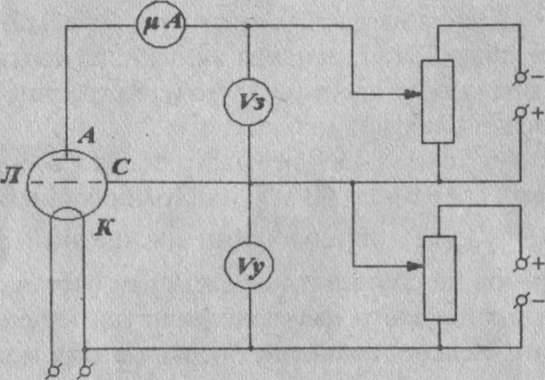
\includegraphics[width=0.7\linewidth]{fig/R1.png} 
        
        \caption{Принципиальная схема экспериментальной установки}
        \label{fig:1}
    \end{figure}
    \begin{figure}[h]
        \centering
        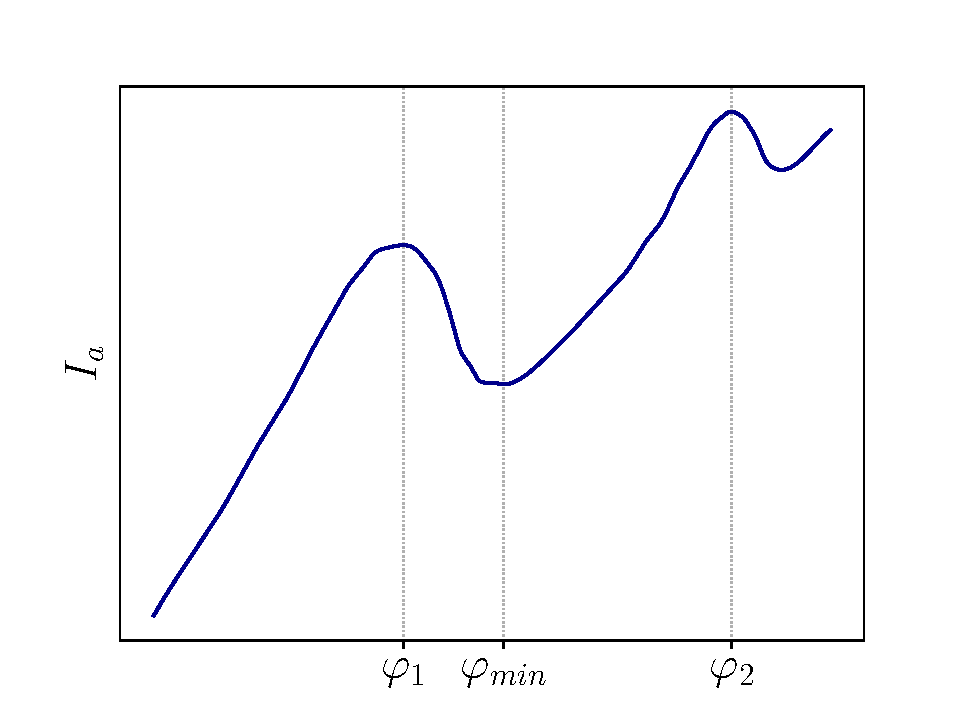
\includegraphics[width=0.7\linewidth]{scripts/pic2} 
        \caption{Анодно-сеточная характеристика газонаполненной лампы}
        \label{fig:2}
    \end{figure}
\end{center}

В ходе выполнения эксперимента снимется анодно-сеточная характеристика газонаполненной лампы, т. е. зависимость анодного 
тока $i_a$ от ускоряющего потенциала $\phi_{\text{y}}$ при постоянном потенциале задержки $\phi_{\text{з}}$. Типичный вид этой характеристики приведен на рис.2.

На начальном участке характеристики по мере увеличения $\phi_y$ наблюдается монотонный рост анодного тока. В этом режиме вылетающие из катода электроны при движении к сетке приобретают сравнительно малую энергию $W_e$ и сталкиваются с атомами газа упруго. При таких столкновениях кинетическая энергия атома изменяется слабо - на величину порядка $$\Delta W\sim W_e\frac{m}{M}\ll W_e,$$ где m и M - массы электрона и атома соответственно, а внутреннее состояние атома не меняется. Поскольку при столкновениях атомы отбирают у электронов лишь незначительную часть энергии, последние, проходя через некоторую эквипотенциальную поверхность с потенциалом $\phi$, имеют энергию, примерно равную $e\phi$ (здесь не учтена начальная скорость вылета электронов с катода).

При $\phi_{y} > \phi_{\text{з}}$ электроны пролетают через сетку, имея энергию, достаточную для преодоления 
задерживающего потенциала, и достигают анода. Как и в обычных электронных лампах, с ростом потенциала сетки $\phi_{y}$ анодный
 ток возрастает. Этот процесс продолжается до тех пор, пока $\phi_{y}$ не достигнет величины
так называемого первого критического потенциала $\phi_{1}$ (его называют также резонансным потенциалом), при котором электроны 
приобретают энергию, достаточную для возбуждения атома. Столкновения электронов, имеющих энергию $e\phi_{1}$, с атомами могут 
происходить неупруго. При этом электрон в процессе столкновения всю свою энергию передает атому. Величина критического
потенциала $\phi_{1}$ связана с разностью энергии возбужденного 
$E_1$, и невозбужденного $E_0$ атомов законом сохранения энергии: $$e\phi_{1}=E_1-E_0.$$

Электроны, потерявшие энергию при неупругих столкновениях, не могут преодолеть задерживающего поля между анодом и сеткой
и "вылавливаются" последней, поэтому анодный ток с дальнейшим ростом 
$\phi_{y}$ уменьшается. Так возникает падающий участок на анодно-сеточной характеристике.

При дальнейшем увеличении $\phi_{y}$ поверхность с потенциалом $\phi_{1}$ (а, следовательно, и область неупругих
соударений) смещается от сетки к катоду. При $\phi_{y} \geqslant \phi_{1}+|\phi_{3}|$ электроны, испытавшие
неупругие соударения на пути к сетке, вновь могут набрать энергию, превышающую $e\phi_{\text{з}}$, и анодный ток опять
возрастает с ростом $\phi_{\text{y}}$. Начиная со значения $\phi_{\text{y}}\geqslant2\phi_{1}$, электроны на своем пути могут дважды неупруго столкнуться с атомами и, потеряв энергию после второго столкновения, не преодолеть задерживающий потенциал. Это приведет к появлению второго провала на анодно-сеточной характеристике. Аналогичным образом происходит падение тока и при более высоких потенциалах $\phi_{n}=n\phi_{1}$.

Таким образом, опыт Франка-Герца убедительно подтверждает справедливость первого постулата Бора: атом действительно поглощает энергию только определенными дискретными порциями.

Франк и Герц, выполнив свои эксперименты с парами ртути, показали, что минимальная энергия, которую способен поглотить атом ртути составляет 4.9 Эв, т.е. величина резонансного потенциала равна 4.9 В. Они установили также, что возбужденные до резонансного уровня атому ртут, переходя в невозбужденное состояние, являются источником ультрафиолетового излучения с длиной волны 2537 \AA. Этот результат находится в полном соответствии со вторым постулатом Бора.

\section{Экспериментальная часть}
В экспериментальной установке используется переделанная манометрическая лампа типа ЛМ-2: ее V-образный катод заменен прямой нитью накала, в результате вся система электродов приобрела цилиндрическую симметрию. Силовые линии электрического поля внутри лампы имеют весьма сложную форму.

Это обусловлено несколькими причинами: во-первых, конструктивными особенностями сетки (шаг её витков соизмерим с расстоянием от сетки до катода и анода); во вторых, наличием отрицательного пространственного заряда у катода (как в обычной электронной лампе) и, наконец, неэквипотенциальностью самой поверхности катода, к концам которого приложено накальное напряжение. В таких условиях, даже экспериментально подобрав оптимальное давление заполняющего лампу газа, на анодно-сеточной характеристике удается получить лишь два хорошо выраженных максимума тока. Но для определения резонансного потенциала этого вполне достаточно.

Рассмотрим качественно процессы, происходящие в лампе. Подлетая к эквипотенциальной поверхности $S_1$ с критическим потенциалом $\phi_1$, электроны имеют энергию, достаточную для возбуждения атома. Однако  неупругие столкновения происходят вблизи $S_1$ случайно в пределах длины свободного пробега электронов $\lambda$, т.е. существует область неупругих столкновений $\Omega$ -
слой, примыкающий к поверхности $S_1$ (в сторону нарастания потенциала) толщиной порядка $\lambda$. С ростом величины $\phi_y$ этот слой вначале появляется у витков сетки.

Энергии электронов, испытывающих соударения в различных точках слоя, могут различаться на величину порядка
$$\Delta W_{\lambda}= e \lambda \dv{\phi}{n},$$
где $\displaystyle \dv{\phi}{n}$ - производная по нормали к $S_1$.

Разброс по энергиям на $\Delta W_{\lambda}$ расширяет максимум анодно-сеточной характеристики и уменьшает крутизну падающего участка.

Проще всего это понять на <<плоской модели>> со сплошной сеткой, проницаемой для электронов. В такой модели электрические поля между сеткой и катодом, сеткой и анодом однородны, а эквипотенциальные поверхности, показанные на рис.\ref{fig:3} штрихованными линиями представляют собой плоскости, параллельные электродам.

\begin{figure}[H]
    \centering
    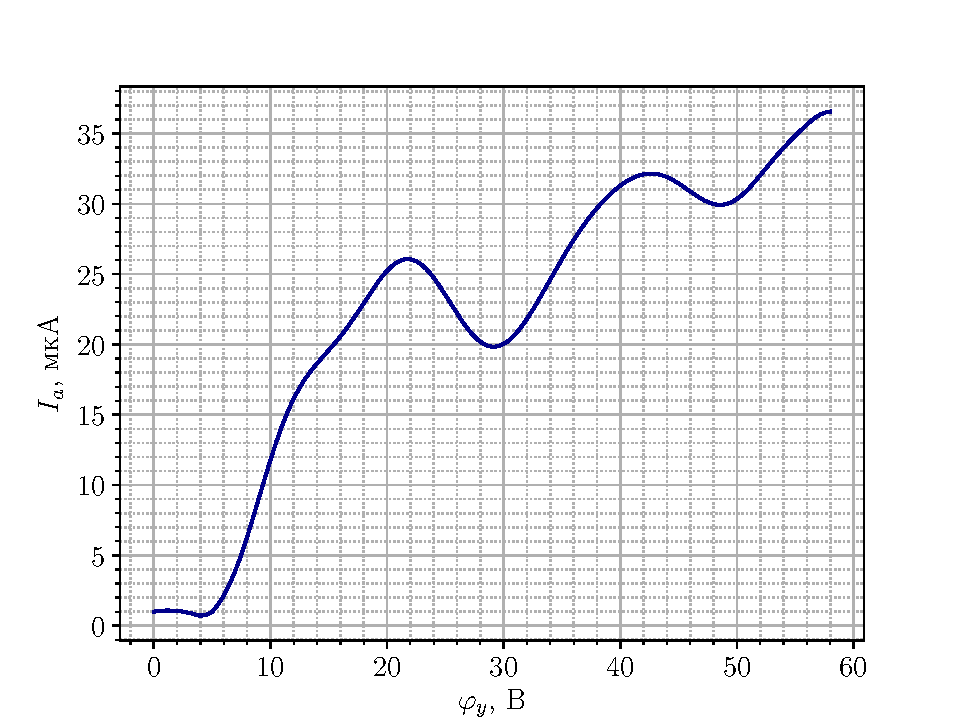
\includegraphics[]{fig/1}
    \caption{Силовые линии электрического поля и эквипотенциальные поверхности между электродами лампы в плоской модели.}
    \label{fig:3}
\end{figure}

Анодный ток будет тем меньше, чем больше неупругих соударений происходит в объеме $\Omega$. В этой модели минимум анодного тока будет наблюдаться тогда, когда поверхность $S_1$ с потенциалом $\phi_1$ сместится от сетки к катоду на длину $\lambda$, т.е. при ускоряющем потенциале на сетке:
\begin{equation*}
      \phi_{min}= \phi_1 +\lambda \dv{\phi}{n}.
\end{equation*}  

Уменьшение величины $\displaystyle \lambda \dv{\phi}{n}$, сужает максимум анодно-сеточной характеристики (см. рис.\ref{fig:2}). Одновременно увеличивается крутизна её падающего участка.

Аналогичная картина будет  и в реальной лампе. Таким образом, экспериментальная погрешность определения критического потенциала оценивается как:
\begin{equation*}
    \Delta \phi \sim \lambda \dv{\phi}{n}
\end{equation*}


Заметим далее, что если на длине свободного пробега электрон может набрать энергию, большую разности энергий двух уровней $E_n-E_1$, то возможно возбуждение всех уровней с
энергией, меньшей $E_n$, и даже ионизация атома, если $E_n-E_1$ больше энергии ионизации. Поэтому уменьшение длины свободного пробега $\lambda$ (за счет увеличения давления газа внутри лампы) позволяет не только увеличить точность определения резонансного потенциала, но и избежать перекрытия различных ступеней возбуждения. С другой стороны, слишком сильное уменьшение $\lambda$ нецелесообразно, т. к. при этом электроны до прихода в область неупругих соударений $\Omega$ испытывают много упругих столкновений, что увеличивает их разброс по энергиям, и, следовательно, уменьшает точность определения резонансного потенциала.

Для некоторых газов, у которых величина резонансного потенциала не сильно отличается от потенциала ионизации, можно, используя эту же лампу, только при относительно больших потенциалах задержки 
($\phi_{3} /\phi_{y} \sim1$), измерить также и потенциал ионизации.

Для этого можно использовать то обстоятельство, что при 
$|\phi_{3}|>{\phi_{y}}$, электроны, эмитированные катодом, не достигают анода, и анодный ток может быть вызван только положительными носителями заряда. В случае $|\phi_{3}|>{\phi_{y}}\geqslant{\phi_{u}}$ наличие анодного тока связано с процессами ионизации электронным ударом в окрестностях сетки. Когда $\phi_{y}$ достигнет значения $\phi_{u}$, у витков сетки появится область неупругих соударений, в которой энергия электронов будет достаточна для ионизации атомов газа, и возникнет ионный ток между сеткой и анодом лампы. В анодной цепи ток в этом случае будет иметь направление, противоположное обычному и для его измерения необходимо произвести <<переполюсовку>> амперметра (заметим, что название <<анод>>\,в этом случае оказывается чисто условным).

Ранее утверждалось, что для точного определения резонансного потенциала необходимо избежать перекрытия различных ступеней возбуждения; а в этом случае электроны на длине свободного пробега должны набирать энергию, не превышающую разности уровней $\text{Е}_{2}-E_{1}$. Для ионизации же необходимо, чтобы энергия, полученная электроном на длине свободного пробега, была бы не меньше $E_{u}-E_1$ ($E_{u}$ - энергия, соответствующая ионизированному атому). Казалось бы, одновременное выполнение этих двух условий невозможно. Но нельзя забывать, что картины электрических полей внутри лампы при определении резонансного потенциала и потенциала ионизации будут совершенно различными. Нетрудно убедиться, что производная $\displaystyle\dv{\phi}{n}$ во втором случае будет существенно выше, следовательно, и электрон в этом случае может набрать на длине свободного пробега существенно большую энергию $$\Delta W_{\lambda}=e\lambda \displaystyle\dv{\phi}{n}.$$

В данной работе в качестве рабочего газа использовался гелий, при этом давление в лампе $\rho$=1.2 мм рт.ст.
\subsection{Определение резонансного уровня}




\begin{figure}[H]
    \centering
    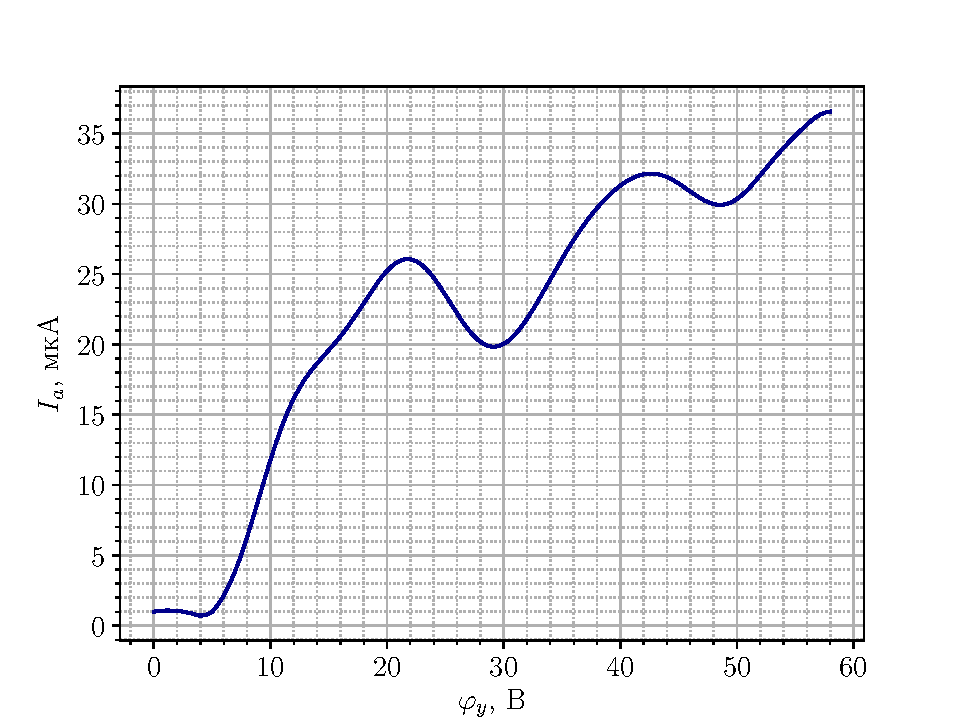
\includegraphics[width=\linewidth]{fig/1}
    \caption{Зависимость анодного тока от ускоряющего потенциала}
    \label{fig:4}
\end{figure}

Напряжение накала $V_{\text{н}}$ = 3 В.

Напряжение задержки $V_{\text{з}}$= 7.5 В.

Резонансный потенциал $\phi_1=21.6\pm 0.75$ Эв.

Потенциал $\phi_2=42.2 \pm 0.75$ Эв.

Разность энергетических уровней $E_1-E_0=e\phi_1=21.6\pm 0.75$ Эв.

Табличное значение $E_1-E_0=21.2$ Эв
\subsection{Определение ионизационного потенциала}
 При разных значениях запирающего потенциала, превышающего потенциал ускорения, была снята зависимость анодного тока от
  ускоряющего потенциала. 



\begin{figure}[H]
    \centering
    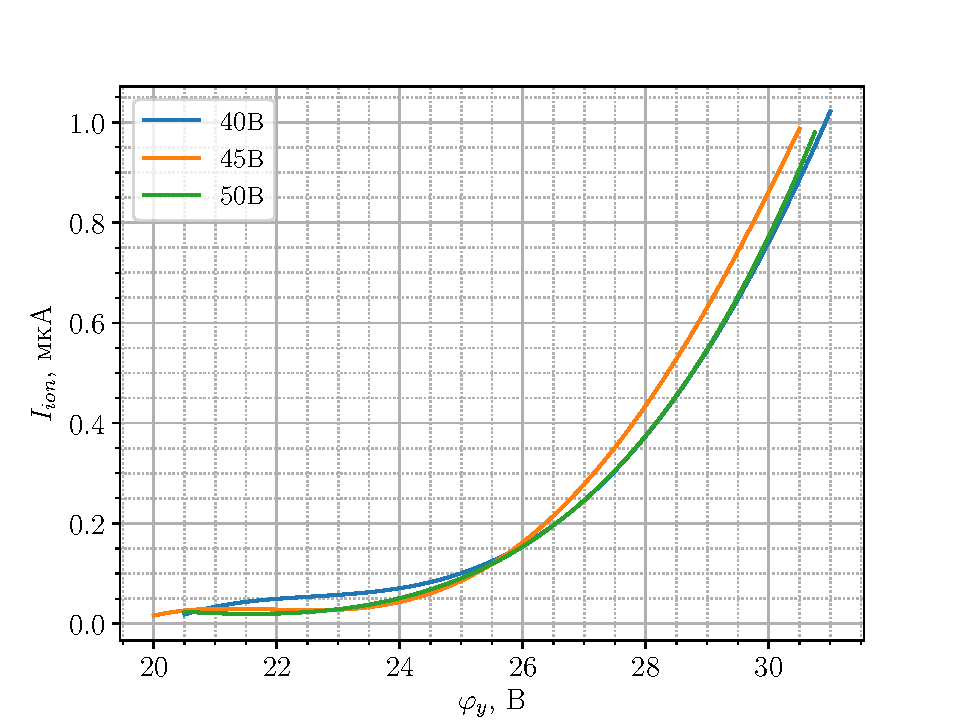
\includegraphics[width=\linewidth]{fig/2}
    \caption{Зависимость ионного тока от ускоряющего потенциала}
    \label{fig:5}
\end{figure}

Потенциал ионизации $\phi_u$ определялся как значительное увеличение анодного тока при повышении ускоряющего
потенциала. При значениях, близких, но меньше $\phi_u$ анодный ток может появляться ввиду разброса электронов по
скоростям при эмитировании с катода. Электроны, обладающие большей начальной скоростью могут ионизировать атом, при том
что большая часть атомов останется не ионизированными. Определенный $\phi_u$ составил $\phi_u=25.7\ \text{Эв}$ 

Для ионизации атомов газа необходимо, чтобы энергия, которую приобретает электрон на длине свободного пробега $\Delta W_{\lambda}=e\lambda \displaystyle\dv{\phi}{n}$
была бы не меньше энергии $E_u-E_1=e(\phi_u-\phi_1)=4.1\text{ Эв}.$ 

\section{Вывод}
В проведенной работе был экспериментально подтвержден вид сеточной характеристики и ионного тока. Были получены значения
$\phi_1$, $\phi_2$ и $\phi_u$, напрямую связанные со свойствами исследуемого газа.
\end{document}